
% Platzhalter für finale Einrückung
\let\levelone\section
\let\leveltwo\subsection
\let\levelthree\subsubsection

\levelone{Nutzerhandbuch \sk}
\label{sec:nutzerhandbuch:sk}
In den nachfolgenden Abschnitten wird die Inbetriebnahme und anschließende Konfiguration eines \sk erläutert.

\leveltwo{Überblick über die verwendete Hardware}
Für den Betrieb des Sensorknotens wird ein Mikrocontroller sowie angeschlossene Sensoren verwendet.
Als Mikrocontroller kommt eine NodeMCU ESP8266 zum Einsatz.
Im Standardaufbau werden zudem ein Nova SDS011 zur Messung von Feinstaub und ein BME280 zur Messung von Temperatur, Luftfeuchte und -druck verwendet.

\levelthree{NodeMCU ESP8266}
Diese Komponente ist das Herzstück der Sensorstation und besitzt neben der CPU ein WLAN Modul.
Dieses Board wird über einen MicroUSB"=Anschluss mit Strom versorgt.
Neben dem MicroUSB"=Anschluss gibt es 30 Pins, um Sensoren und/oder Aktuatoren anzuschließen.

\levelthree{SDS011}
Der Feinstaubsensor "Nova SDS011", der in den Sensorknoten eingebaut ist, misst Feinstaub der Partikelgröße PM 2,5 und PM 10.
Dabei wird das Prinzip der Laserstreuung ausgenutzt, indem die Partikel gemessen werden, die durch den gemessenen Bereich fliegen.
Die Laserstrahlen werden dann in elektrische Signale umgewandelt, die dann bereitgestellt werden können.
Dabei wird die Luft mit einem kleinen Lüfter durch den Bereich befördert.

\levelthree{BME280}
Der BME280 ist ein Sensor zur Messung der Temperatur, Luftfeuchtigkeit und Luftdruck.
Er eignet sich zum Anschluss an verschiedene Boards wie Arduino"=Boards oder den Raspberry Pi.
Der Sensor ist ideal zum Betrieb einer Wetterstation.

\leveltwo{Aufbau von einem \sk}
Die benötigten Komponenten, um einen \sk aufbauen zu können, sind in \Fig{skcomponents} abgebildet.

\begin{figure}[htb]
	\begin{minipage}{0.6\textwidth}
		\centering
		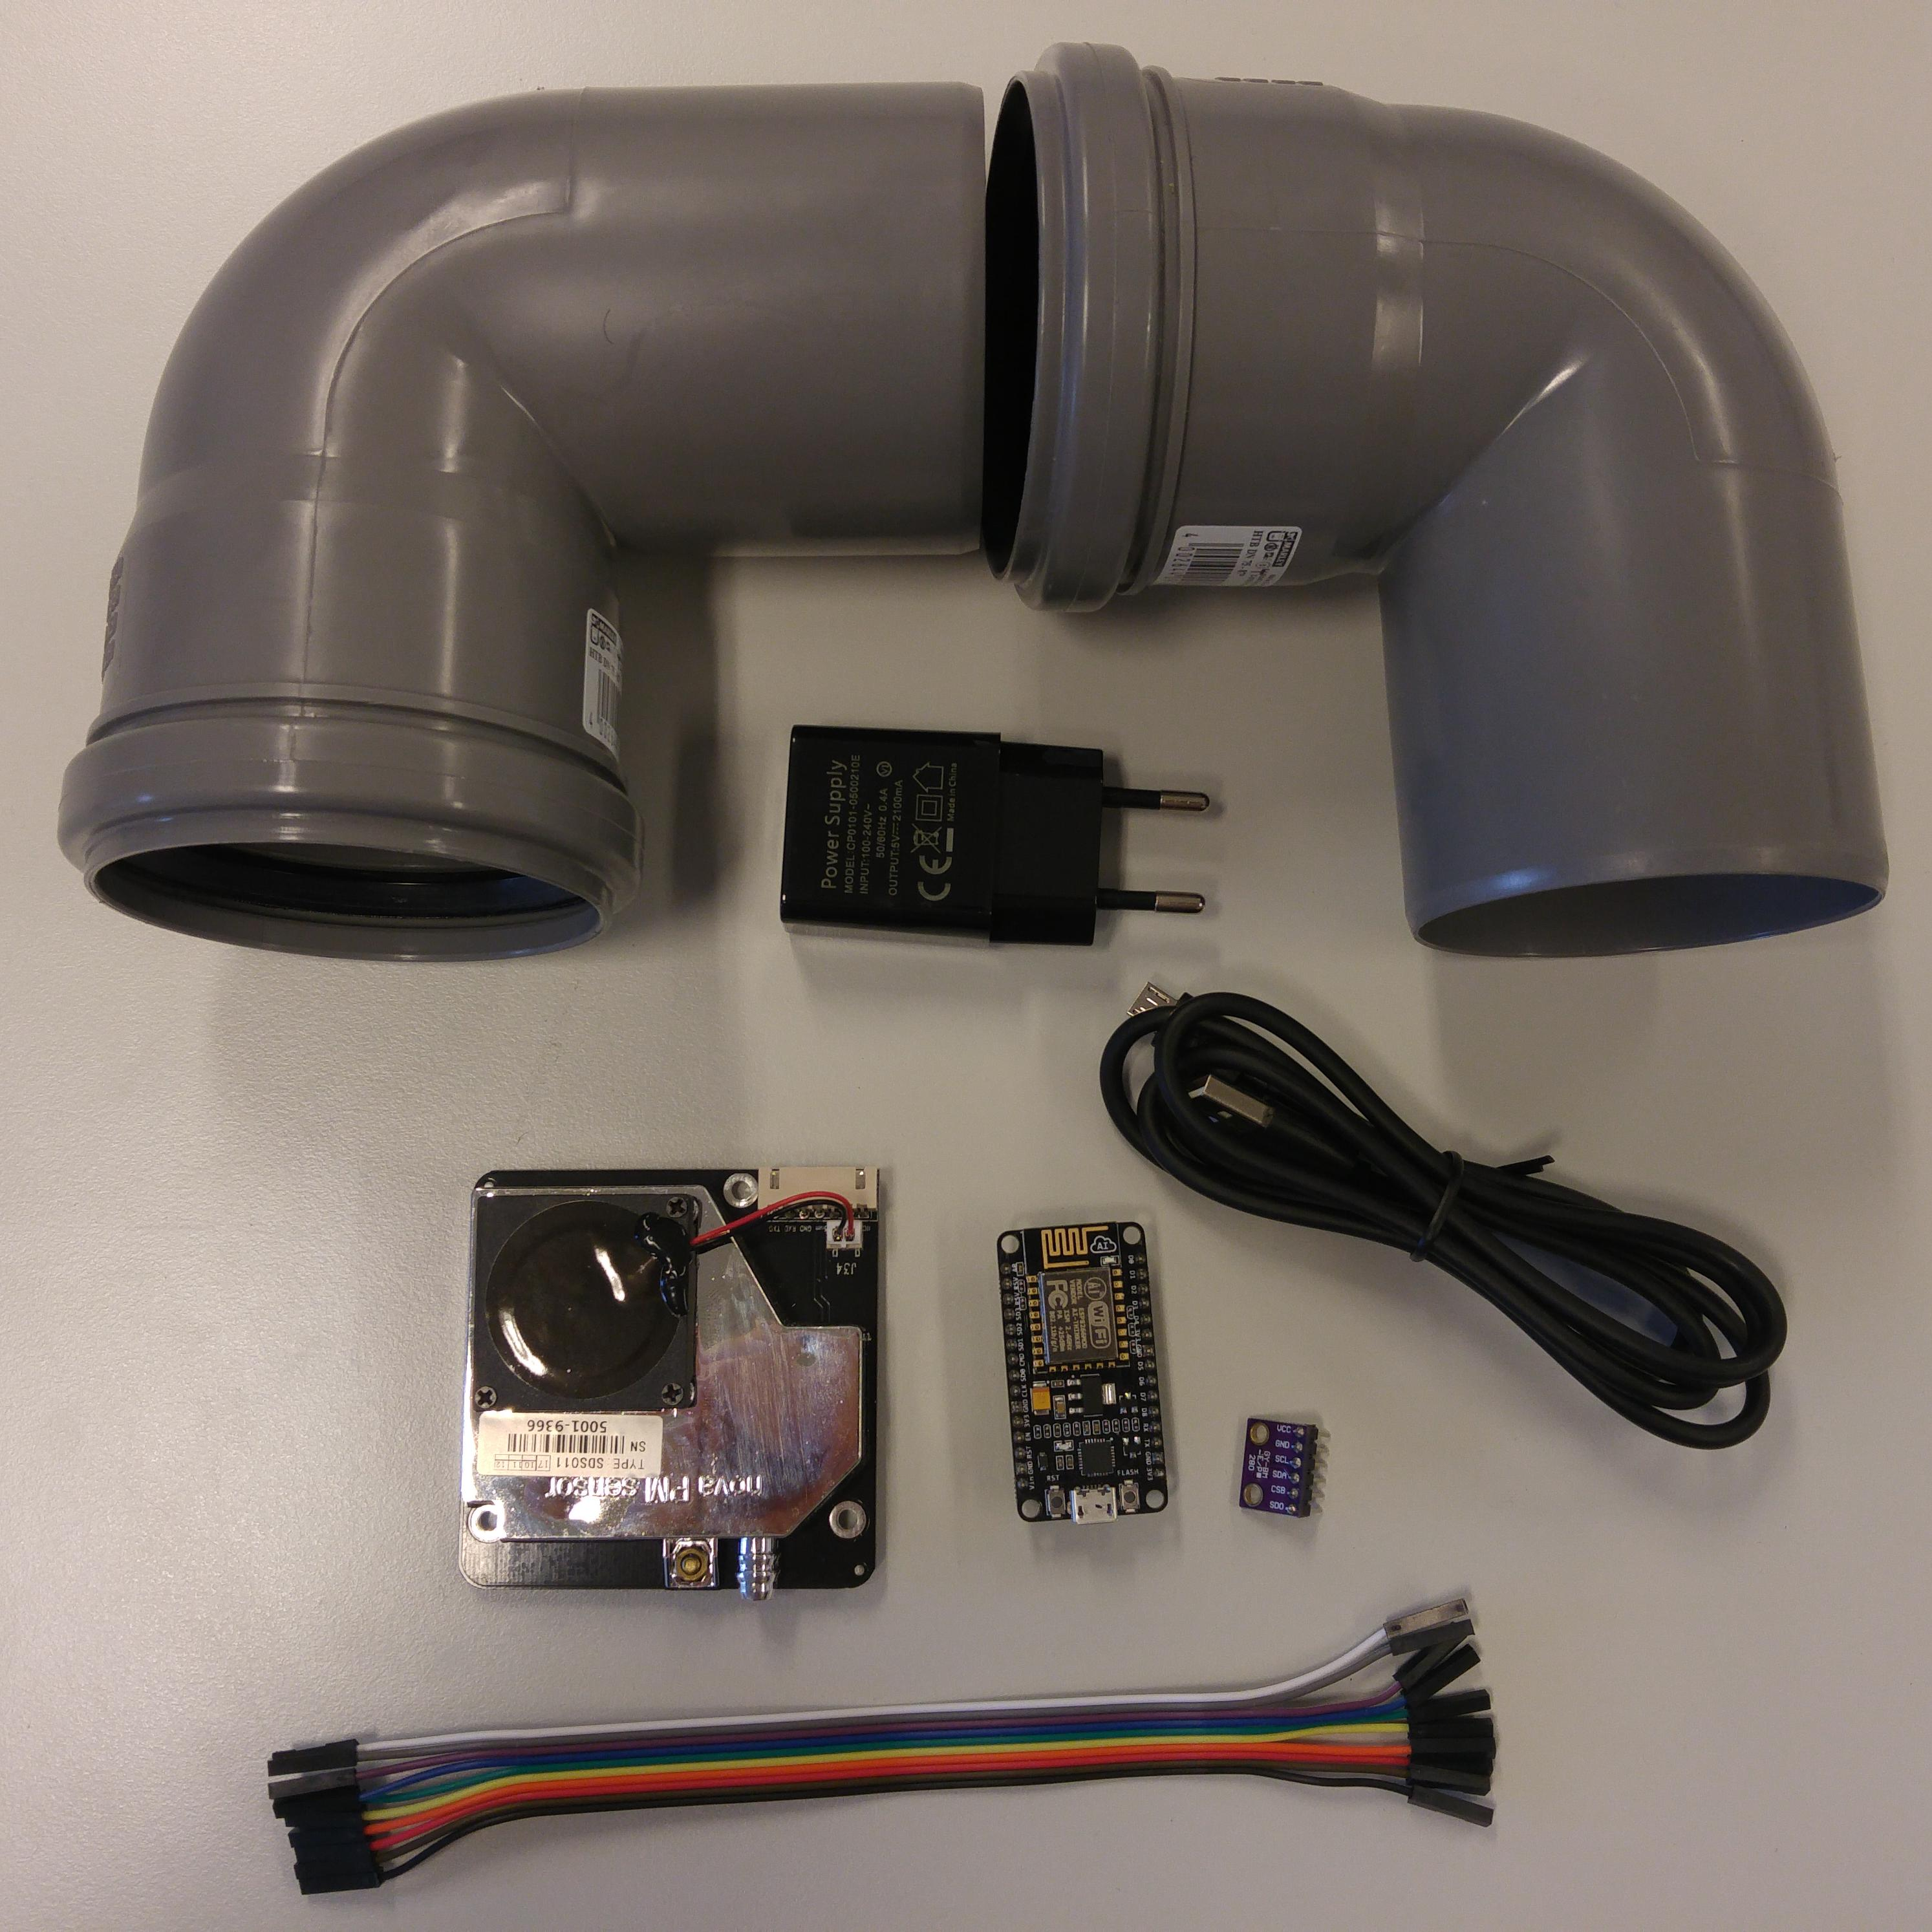
\includegraphics[width=\textwidth]{./ressourcen/SK-HardwareUeberblick.jpg}
	\end{minipage}
	\begin{minipage}{0.35\textwidth}
		\begin{itemize}
			\item 2x \SI{90}{^\circ} HT"=Bögen
			\item \SI{5}{V}"=Netzteil
			\item Micro"=USB"=Kabel
			\item SDS011
			\item NodeMCU
			\item BME280
			\item Jumper"=Kabel
			\item Schlauch mit \SI{6}{mm} Innendurchmesser
			\item \textbf{Optional:} 
			\begin{itemize}
				\item Kabelbinder zur Montage
			\end{itemize}
		\end{itemize}
	\end{minipage}
	\caption{Die benötigten Komponenten für einen \sk}
	\label{fig:skcomponents}
\end{figure}

Der Standardaufbau eines Sensorknotens kann aus \Fig{skwiringdefault} entnommen werden:

\begin{figure}[htb]
	\centering
	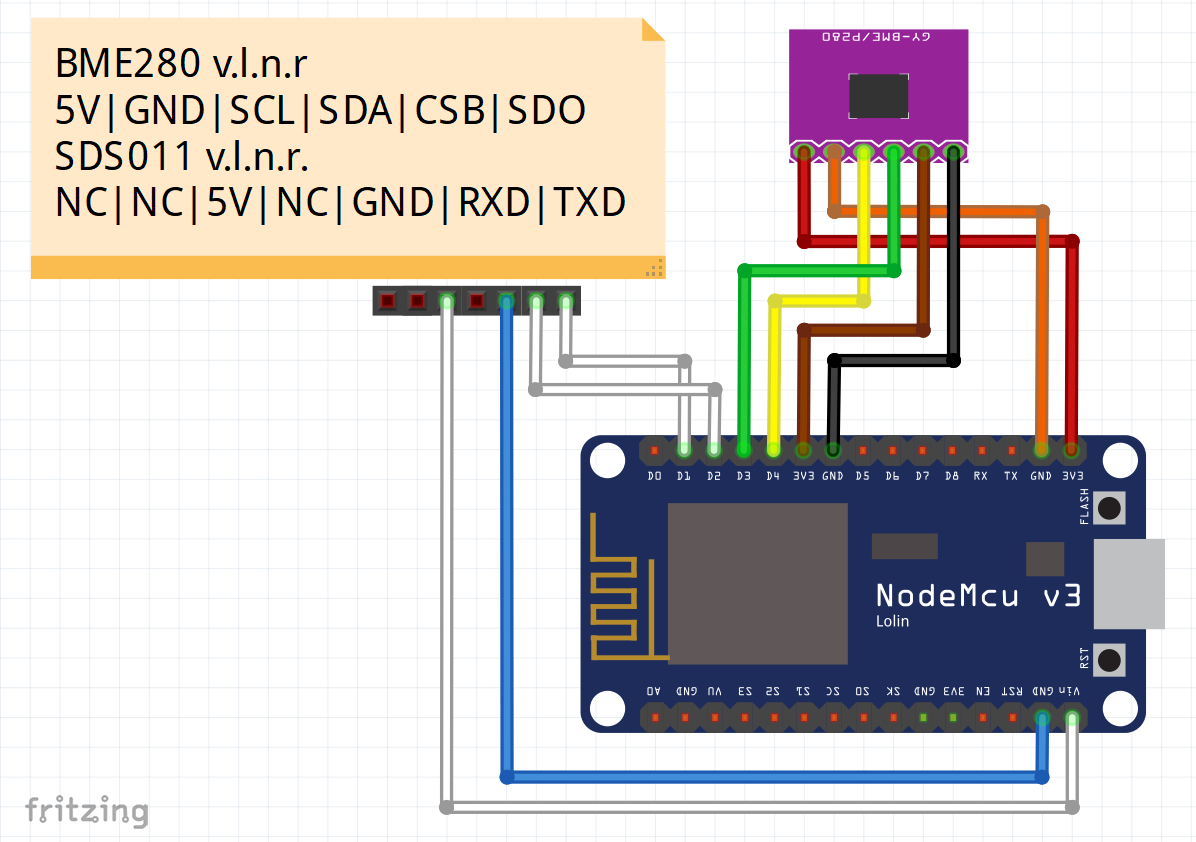
\includegraphics[width=0.8\textwidth]{./ressourcen/Prod_Verdrahtungsplan}
	\caption{Der Standard"=Verdrahtungsplan für den \sk}
	\label{fig:skwiringdefault}
\end{figure}

Beim Aufbau ist auf die korrekte Belegung der Pins zu achten. Obiges Bild gilt als Anschlussplan für die Standardkonfiguration.
Sollen andere Pins der NodeMCU verwendet werden, so muss dies der Software über eine angepasste Konfiguration mitgeteilt werden.

Nach dem Verkabeln der Komponenten können diese in die HT"=Bögen gesteckt werden.
Dabei ist auf die korrekte Ausrichtung des SDS011 zu achten, da dieser mit dem Lüfter nach unten montiert werden muss, wie in \Fig{skpositionsds011} gezeigt ist.

\begin{figure}[!htb]
	\centering
	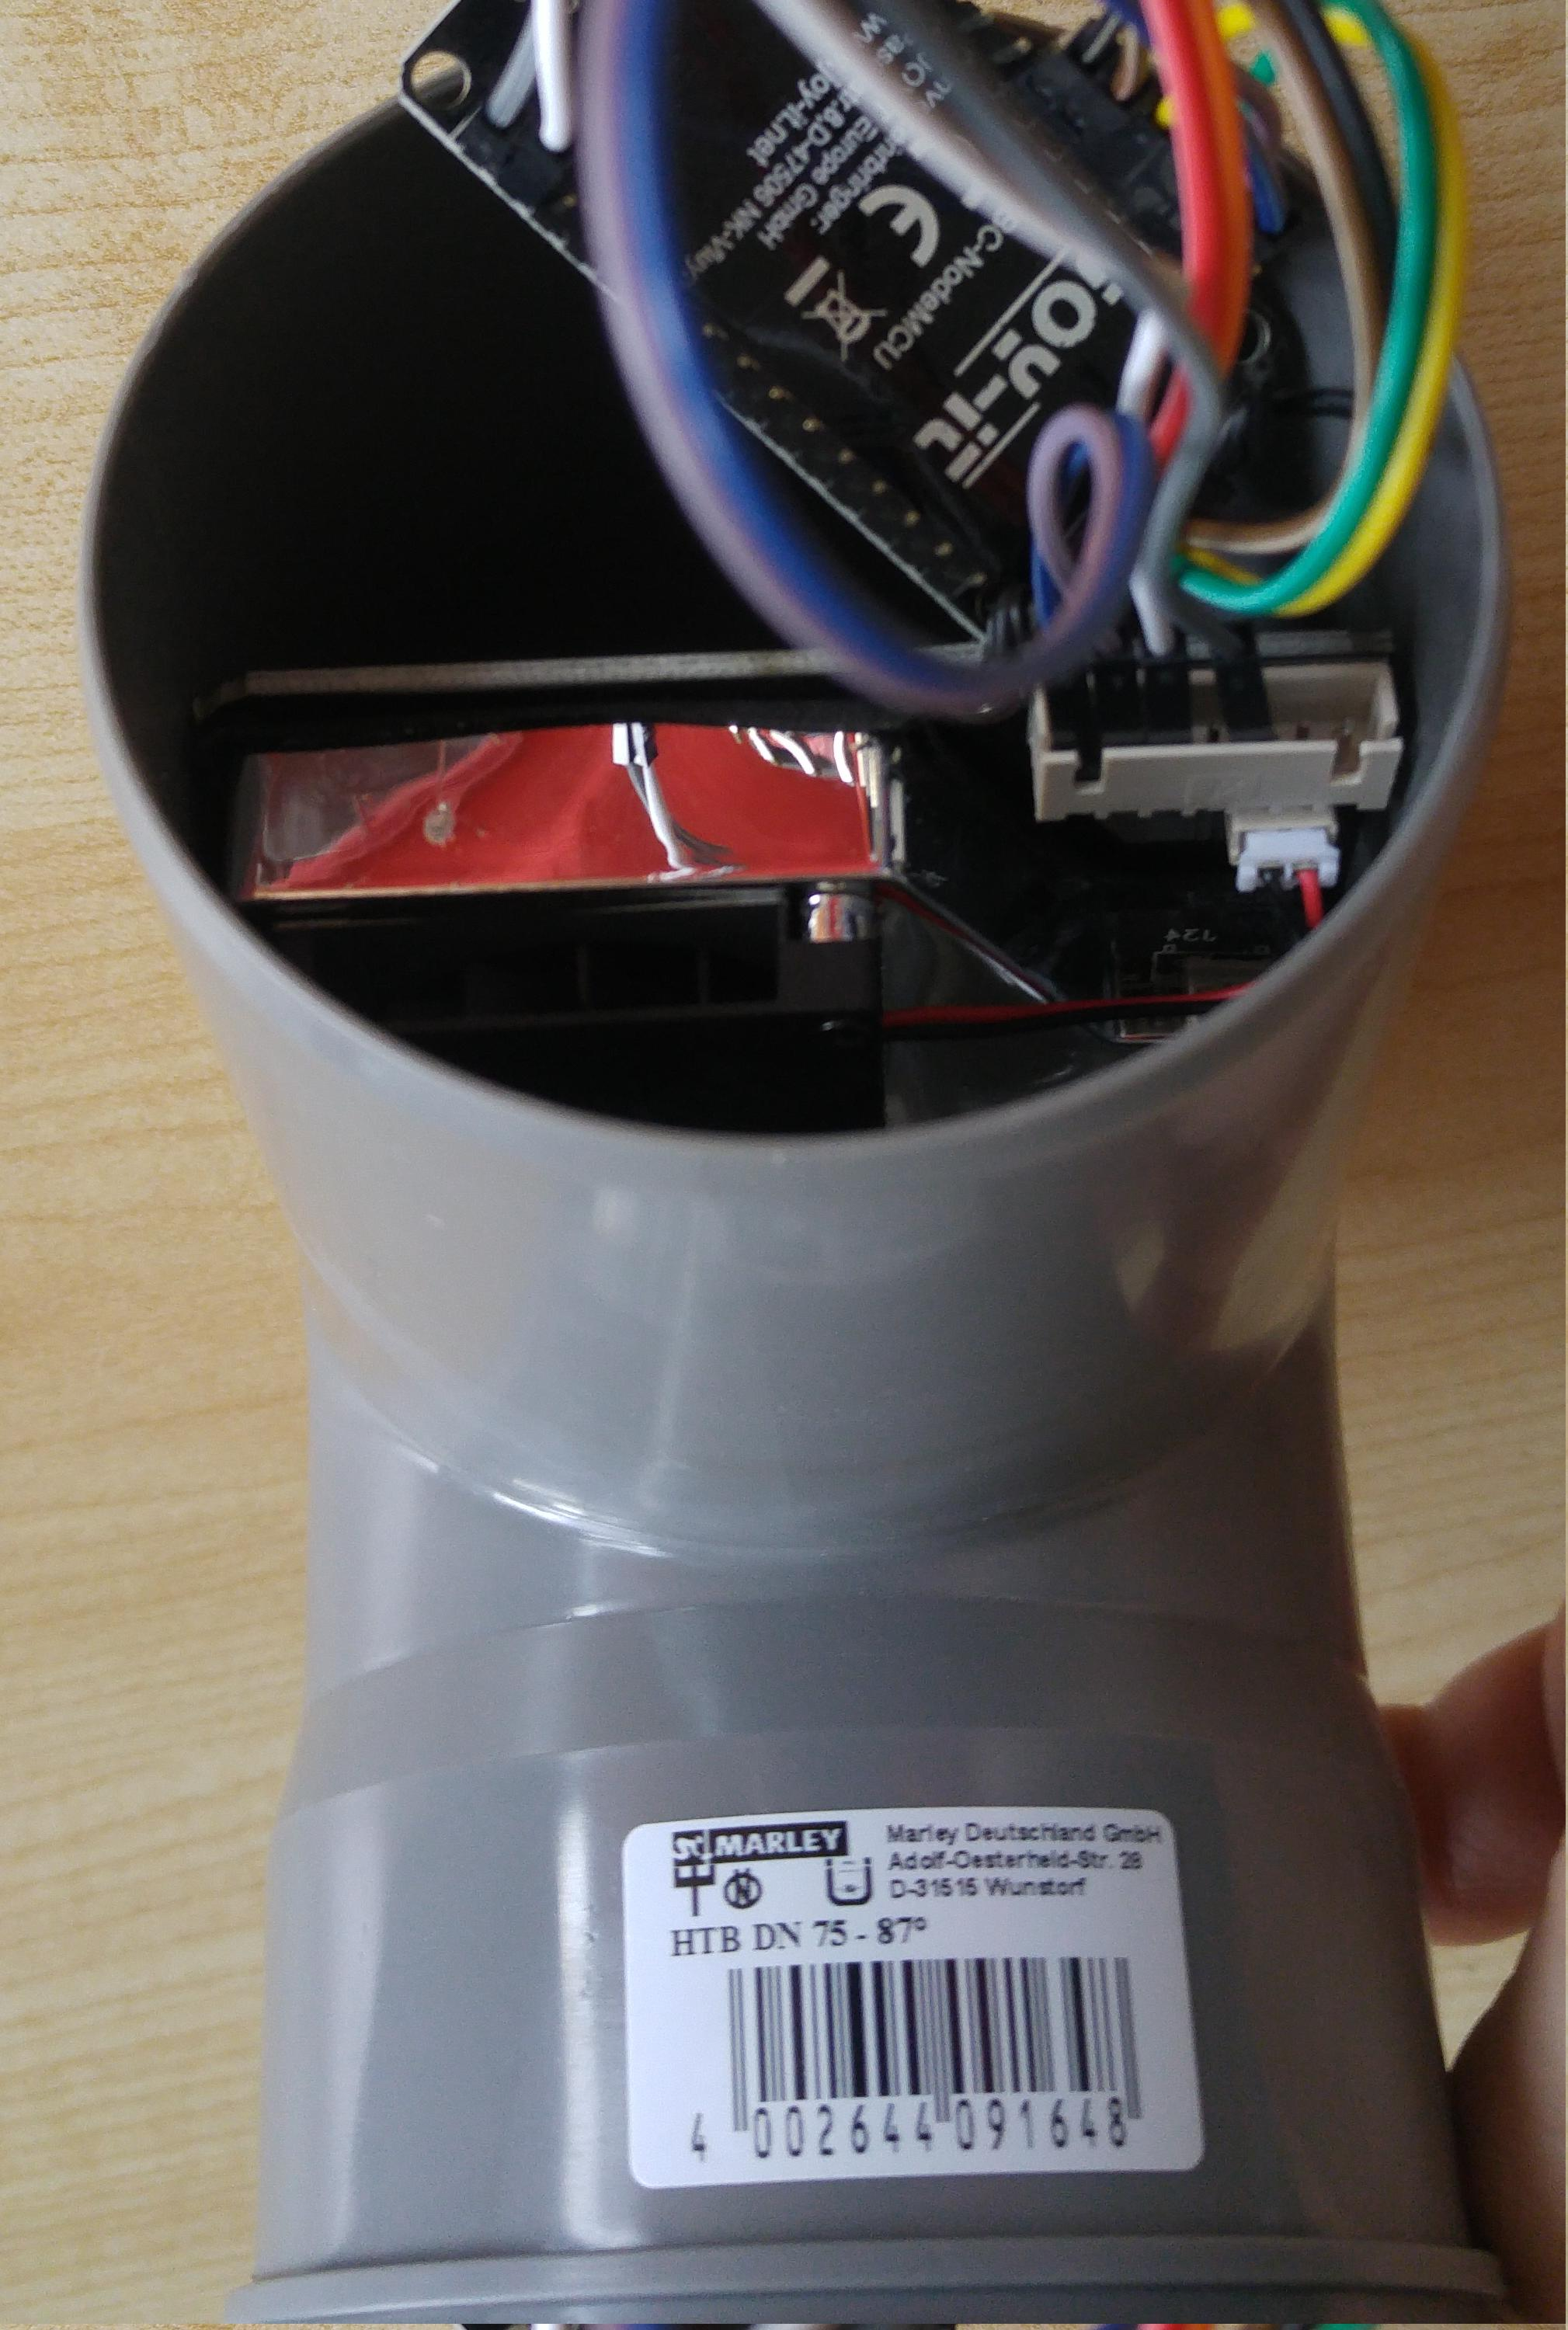
\includegraphics[width=0.6\textwidth]{./ressourcen/SK_AusrichtungSDS.jpg}
	\caption{Position des SDS011 innerhalb der HT"=Bögen}
	\label{fig:skpositionsds011}
\end{figure}


\leveltwo{Aufspielen der Firmware}
Nach dem Aufbau eines \sk geschieht das Aufspielen der Firmware über ein eigens in der \pg entwickeltes Installationstool (nur für Microsoft Windows).
Dieses kann über folgenden Link bezogen werden: \url{https://pg-rio-uis.informatik.uni-oldenburg.de/mitmachen}\footnote{\url{https://pg-rio-uis.informatik.uni-oldenburg.de/assets/tools/PGRIO-SK-Config-Tool.exe}}
\FloatBarrier

Nach dem Starten des Installationstools erscheint das Registrierungs- bzw. Anmeldeformular, abgebildet in \Fig{skitool01}.
\begin{figure}[!htb]
	\centering
	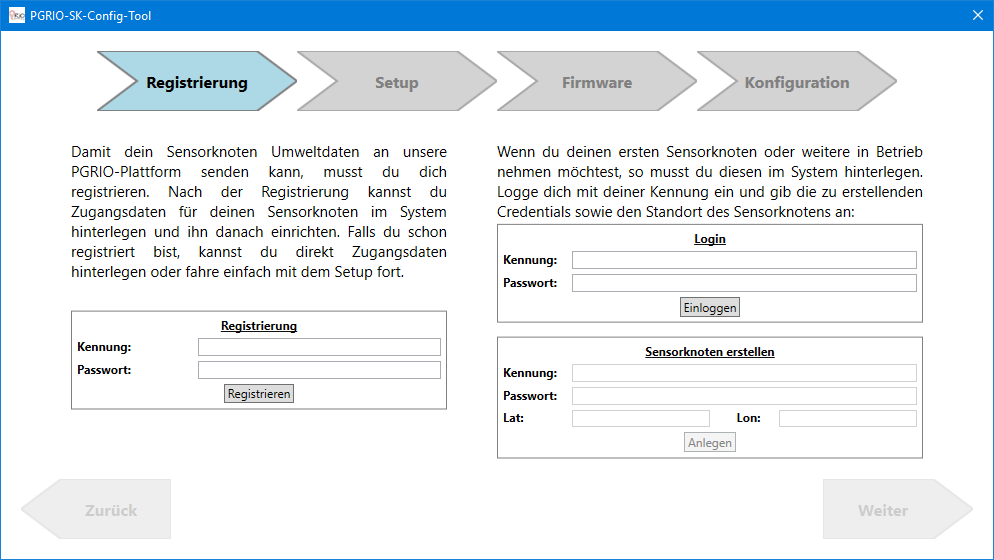
\includegraphics[width=0.8\textwidth]{./ressourcen/i-tool/Registrierung}
	\caption{Die Startseite des Installationstool}
	\label{fig:skitool01}
\end{figure}
Hier kann ein neuer Benutzer (Kennung und Passwort) angelegt werden, der den Eigentümer des \sk repräsentiert.
Mit dieser Nutzerkennung kann dann nach dem Einloggen ein neuer \sk angelegt werden.
Dabei ist zu beachten, dass die Kennung des Sensorknotens mit dem Präfix \textit{pgrio-} beginnen muss.

\begin{mdframed}[frametitle=Weitere Hinweise]
	\begin{minipage}{\linewidth}
	    \begin{itemize}
	        \item Es ist darauf zu achten, dass in der Kennung, sowie dem Passwort keine Sonderzeichen verwendet werden dürfen.
	        \item Fehleingaben werden vom Installationstool abgefangen und durch eine Meldung im unteren Bereich angezeigt.
	        \item Bei länger andauernden Operationen wird ein Ladebildschirm eingeblendet.
	        \item Bei Problemen mit dem Installationstool sollte frühzeitig ein Ansprechpartner der \pg kontaktiert werden.
	    \end{itemize}
	\end{minipage}
\end{mdframed}

Ist der \sk erfolgreich angelegt, erfolgt mit einem Klick auf \PicDet{Weiter} das Setup der Seriellen Verbindung.
Dies ist in \Fig{skitool02} abgebildet.
\begin{figure}[!htb]
    \centering
    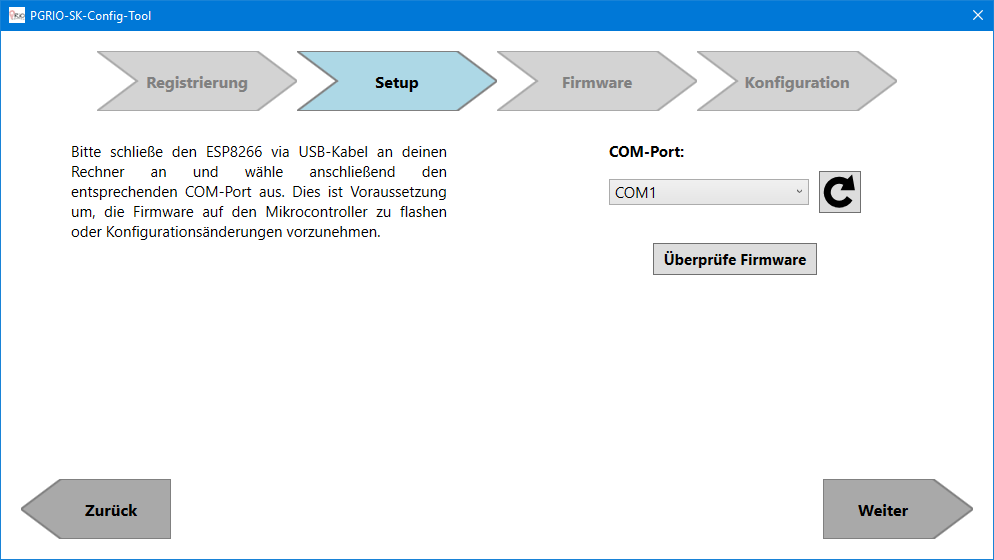
\includegraphics[width=0.8\textwidth]{./ressourcen/i-tool/Setup}
    \caption{Auswahl des Com"=Ports im Installationstool}
    \label{fig:skitool02}
\end{figure}
Hier kann der \PicDet{Com"=Port} ausgewählt werden, mit dem die Verbindung zum \sk aufgebaut werden soll.
Mit dem Button \PicDet{Überprüfe Firmware} kann darüber hinaus überprüft werden, ob bereits eine Firmware im Rahmen dieser \pg auf den \sk aufgespielt worden ist.

\begin{mdframed}[frametitle=Hinweis]
	\begin{minipage}{\linewidth}
    	Falls die Verbindung mit dem \sk über keinen \PicDet{Com"=Port} erfolgreich ist, oder kein \PicDet{Com"=Port} zur Auswahl steht, sollten die verwendeten Treiber für die NodeMCU überprüft werden.
	\end{minipage}
\end{mdframed}

Ist die Verbindung zum \sk erfolgreich hergestellt, kann über einen Klick auf den \PicDet{Weiter}"=Button die Firmware"=Seite aufgerufen werden.
Diese ist in \Fig{skitool03} abgebildet.
\begin{figure}[!htb]
	\centering
	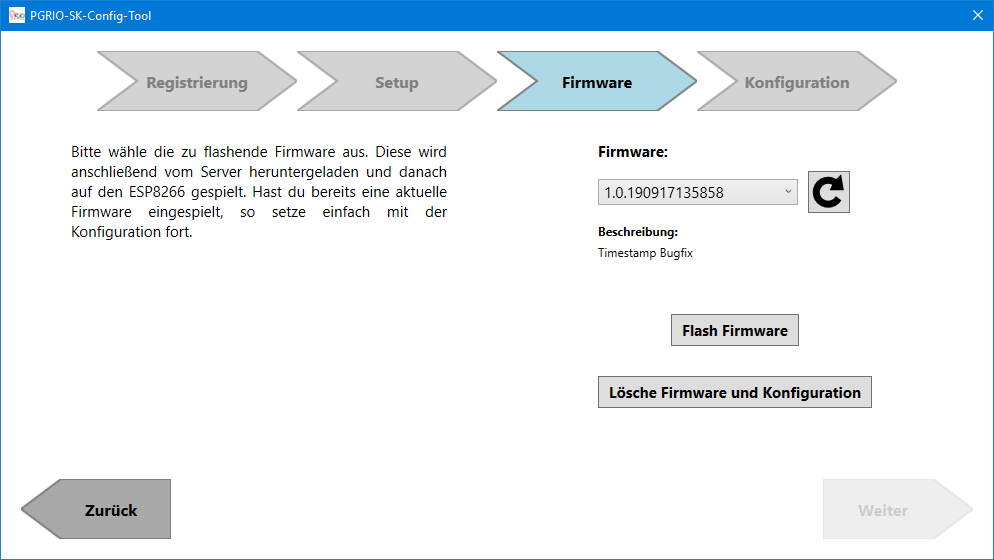
\includegraphics[width=0.8\textwidth]{./ressourcen/i-tool/Firmware}
	\caption{Flashen der \skfw im Installationstool}
	\label{fig:skitool03}
\end{figure}
Hier kann über einen Klick auf den Button \PicDet{Flash Firmware} die Firmware auf den \sk aufgespielt werden.
Zu Testzwecken kann darüber hinaus auch eine spezifische Firmware"=Version über die Auswahl"=Box aufgespielt werden.

\begin{mdframed}[frametitle=Hinweis]
	\begin{minipage}{\linewidth}
    	Sollte bei der späteren Konfiguration etwas fehlschlagen, sodass der \sk nicht mehr über das Installationstool konfiguriert werden kann, kann der gesamte \sk über den Button \PicDet{Lösche Firmware und Konfiguration} in den Werkszustand zurückgesetzt werden.
   \end{minipage}
\end{mdframed}

Sobald die Firmware auf den \sk aufgespielt ist, muss die NodeMCU über den Reset-Knopf neugestartet oder kurzzeitig vom PC getrennt und neu verbunden werden. Nach ca. fünf Sekunden kann über einen Klick auf den \PicDet{Weiter}"=Button die Konfigurations"=Seite aufgerufen werden.
Diese ist in \Fig{skitool05} abgebildet.
\begin{figure}[!htb]
	\centering
	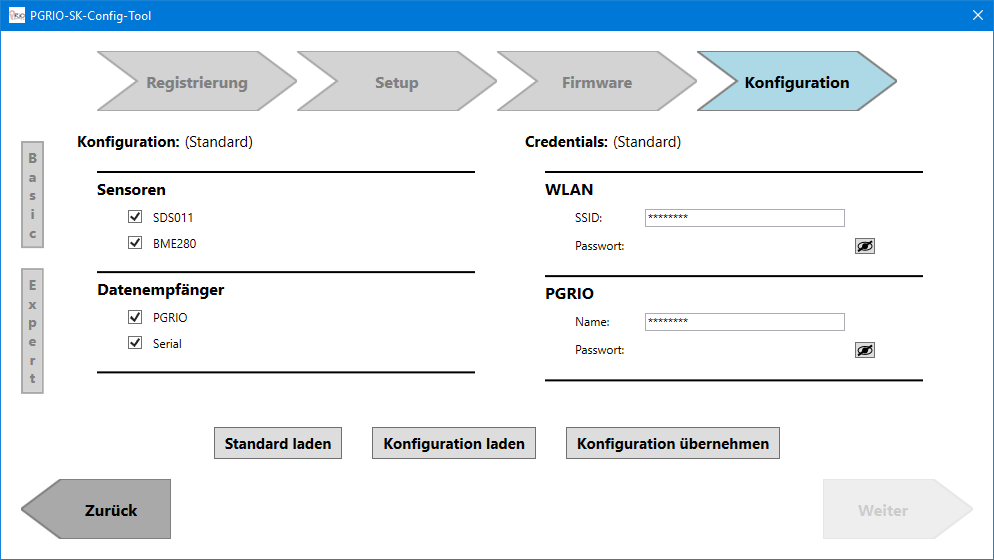
\includegraphics[width=0.8\textwidth]{./ressourcen/i-tool/Konfiguration_basic}
	\caption{Die einfache Konfiguration im Installationstool}
	\label{fig:skitool05}
\end{figure}
Hier kann die angeschlossene Hardware konfiguriert werden, sowie die Zugangsdaten zum WLAN und der IoT"=Plattform (Kennung von der Registrierungs"=Seite) eingegeben werden.
Über einen Klick auf den Button \PicDet{Konfiguration übernehmen} werden diese auf den \sk gespeichert.

\begin{mdframed}[frametitle=Weitere Hinweise]
	\begin{minipage}{\linewidth}
	    \begin{itemize}
	        \item Über den Button \PicDet{Standard laden} kann die Standardkonfiguration wiederhergestellt werden. Diese wird jedoch erst über einen Klick auf den Button \PicDet{Konfiguration übernehmen} gespeichert.
	        \item Über den Button \PicDet{Konfiguration laden} kann eine bereits gespeicherte Konfiguration vom \sk geladen werden.
	        \item Über einen Klick auf den Button \PicDet{Expert} kann in den Expertenmodus gewechselt werden. Dieser wird in \Fref{sec:skitoolExpert} beschrieben.
	    \end{itemize}
	\end{minipage}
\end{mdframed}

\leveltwo{Erweiterte Konfiguration}
\label{sec:skitoolExpert}
Im Experten"=Modus des Installationstools (siehe \Fig{skitool06}) kann die Konfiguration als \filename{.json}"=Datei editiert werden.

\begin{figure}[htb]
	\centering
	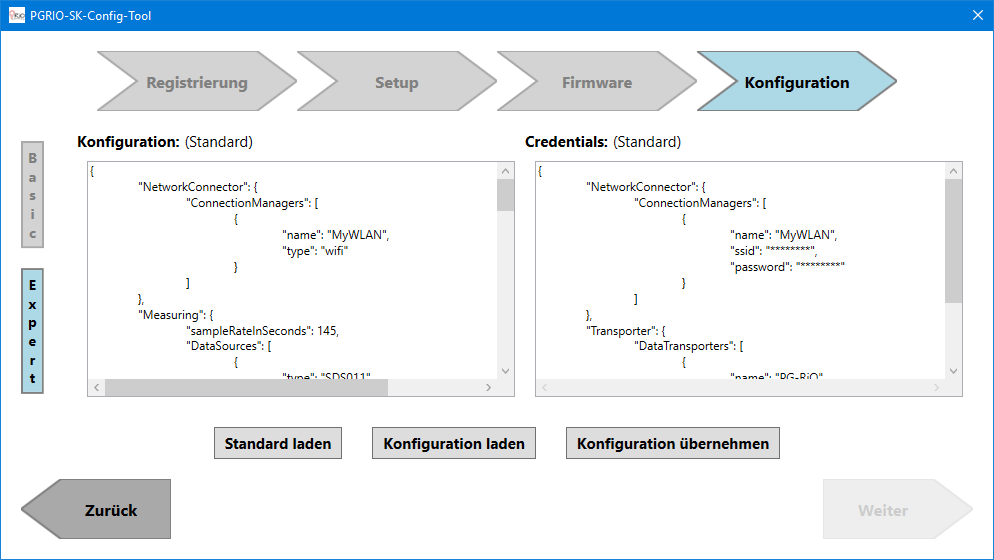
\includegraphics[width=0.8\textwidth]{./ressourcen/i-tool/Konfiguration_expert}
	\caption{Die erweiterte Konfiguration im Installationstool}
	\label{fig:skitool06}
\end{figure}

Dabei können weitergehende Einstellungen vorgenommen werden, die über die einfache Inbetriebnahme eines \sk hinausgehen.

Die Standardkonfiguration sieht dabei wie folgt aus:

\begin{lstlisting}[language=json,basicstyle=\footnotesize]
{
  "NetworkConnector": {
    "ConnectionManagers": [
      {
        "name": "MyWLAN",
        "type": "wifi"
      }
    ]
  },
  "Measuring": {
    "sampleRateInSeconds": 145,
    "DataSources": [
      {
        "type": "SDS011",
        "sdsTxPin": "D1",
        "sdsRxPin": "D2"
      },
      {
        "type": "BME280",
        "bmeSdaPin": "D3",
        "bmeSclPin": "D4"
      }
    ]
  },
  "MeasurementSender": {
    "DataSinks": [
      {
        "type": "PG-RiO",
        "transporterName": "PG-RiO",
        "transformerWhitelist": [
          "ALL"
        ]
      },
      {
        "type": "SerialDump",
        "transformerWhitelist": [
          "ALL"
        ]
      }
    ]
  },
  "Transporter": {
    "DataTransporters": [
      {
        "type": "MQTT_TLS",
        "hostOrIp": "pg-rio-iot.informatik.uni-oldenburg.de",
        "port": 8883,
        "publicKey": "pg-rio-iot",
        "name": "PG-RiO"
      },
      {
        "type": "HTTPS",
        "hostOrIp": "pg-rio-sensors-update.informatik.uni-oldenburg.de",
        "port": 443,
        "publicKey": "pg-rio-sensors-update",
        "name": "PG-RiO-Update"
      }
    ]
  },
  "TimeManager": {
    "TimeSyncStrategies": [
      {
        "type": "NTP",
        "serverName": "pool.ntp.org"
      }
    ]
  },
  "Updater": {
    "cyclic": {
      "transporterName": "PG-RiO-Update",
      "intervalInHours": 24
    }
  },
  "StatusInformation": {
    "sendIntervalInSeconds": 600,
    "transporterName": "PG-RiO"
  }
}
\end{lstlisting}

Die Standardcredentials sieht wie folgt aus:

\begin{lstlisting}[language=json,basicstyle=\footnotesize]
{
  "NetworkConnector": {
    "ConnectionManagers": [
      {
        "name": "MyWLAN",
        "ssid": "********",
        "password": "********"
      }
    ]
  },
  "Transporter": {
    "DataTransporters": [
      {
        "name": "PG-RiO",
        "user": "********",
        "password": "********"
      }
    ]
  }
}
\end{lstlisting}

In den weiteren Abschnitten werden die Einträge weiter erläutert.

\levelthree{NetworkConnector}
Im Bereich NetworkConnector werden verschiedene Verbindungsoptionen für die NodeMCU angegeben, damit er eine Internet"=Verbindung verfügbar hat und gemessene Werte an die IoT"=Plattform senden kann.
In diesem Falle wird ein \textit{ConnectionManager} vom Typ \textit{wifi} mit Namen \textit{MyWLAN} angegeben.
Die Credentials dazu werden mit der selben Struktur in der \filename{credentials.json} passend hinterlegt.
Das Mapping erfolgt dabei über das Attribut \textit{name}.
Diese müssen entsprechend des verfügbaren WLANs angepasst werden.

\levelthree{Measuring}
Im Measuring wird das Messverfahren konfiguriert.
Es werden das Messintervall, sowie die angeschlossenen Sensoren (\textit{DataSources}) konfiguriert.
Aktuell werden die Sensoren \textit{SDS011} und der \textit{BME280} unterstützt.
Für den SDS011 muss angegeben werden, mit welchen Pins der NodeMCU sein TX- sowie RX"=Pin verbunden sind und für den BME280 die zugehörigen Pins seines SDA- sowie SCL"=Pins.
Darüberhinaus können Offsets für die Messwerte angegeben werden.
Wird bei einer Kalibrierung festgestellt, dass der gemessene Wert für beispielsweise PM2.5 systematisch um \SI{5}{\micro g/m^3} vom tatsächlichen Wert abweicht, so kann dies entsprechend konfiguriert werden.
Dabei werden die Offsets für die PM"=Werte über die Schlüssel \textit{offsetPM2.5} bzw. \textit{offsetPM10} in \SI{0,1}{\micro g/m^3} angegeben und die des BME280 über die Schlüssel \textit{offsetTemperature} in \SI{0,01}{^{\circ}C}, \textit{offsetPressure} in \SI{0,01}{hPa} sowie \textit{offsetHumidity} in \SI{0,01}{\%}.

\levelthree{MeasurementSender}
Hier werden die Ziele (\textit{DataSinks}) für die gemessenen Umweltdaten definiert.
Oben wird eine DataSink vom Typ \textit{PG"=RiO} konfiguriert, mit der Messdaten im PG"=RiO"=Format aufbereitet werden, damit sie von der IoT"=Plattform verstanden werden.
Zudem wird der verwendete DataTransporter zum Versenden der Daten über seinen Namen angegeben.

\begin{mdframed}[frametitle=Hinweis]
	\begin{minipage}{\linewidth}
		Die Typen der DataSink und des DataTransporters müssen kompatibel sein, siehe \Fref{sec:userhb:compdsdt}.
	\end{minipage}
\end{mdframed}

Darüberhinaus wird eine Liste der verwendeten DataSources dieser DataSink angegeben.
Das Schlüsselwort \textit{ALL} bedeutet, dass alle verfügbaren Sensoren verwendet werden.

\levelthree{Transporter}
Unter Transporter werden mehrere \textit{DataTransporters} angegeben.
Diese sind für den Datenverkehr verantwortlich.
Z.B. muss ein DataTransporter angegeben werden, mit dem die gemessenen Umweltwerte versendet werden können.
Im Standardfall wird ein \textit{MQTT}"=DataTransporter konfiguriert, der mit dem Host \url{pg-rio-iot.informatik.uni-oldenburg.de} verbunden wird.
Dazu muss in der \filename{credentials.json} ein gültiger User und ein Passwort angegeben werden, um sich am Server zu authentifizeiren.
Das Mapping erfolgt dabei wieder über das Attribut \textit{name}.
\begin{mdframed}[frametitle=Hinweis]
	\begin{minipage}{\linewidth}
		\begin{itemize}
			\item Für den \text{MQTT}"=DataTransporter auf dem Host \url{pg-rio-iot.informatik.uni-oldenburg.de} muss der Public"=Key vom Server mit dem in der Firmware hinterlegten Key übereinstimmen.
			\item Der Port ist in dieser Konstellation fix auf 8884 festgelegt.
		\end{itemize}
	\end{minipage}
\end{mdframed}

\levelthree{TimeManager}
Aus Umweltdaten werden Umweltinformationen, wenn sie u.a. einen Zeit- und Raumbezug haben.
Damit die gemessenen Werte also dem tatsächlichen Zeitpunkt der Messung zugeordnet werden können, muss der Mikrocontroller seine Systemzeit synchronisieren.
Dazu werden \textit{TimeSyncStrategies} verwendet.
Im obigen Fall wird eine \textit{NTP}"=Strategie angegeben, mit deren Hilfe die Systemzeit mit dem angegebenen NTP"=Server (hier \url{pool.ntp.org}) synchronisiert wird.

\levelthree{Updater}
Hier wird das automatische Update konfiguriert.
Aktuell kann ausschließlich eine zyklische Überprüfung angegeben werden.
Dort wird das Prüf"=Intervall in Stunden und der zugehörige DataTransporter angegeben, über den auf Updates geprüft wird. Mittels selben DataTransporter werden vorhandene Updates auch heruntergeladen.
\begin{mdframed}[frametitle=Hinweis]
	\begin{minipage}{\linewidth}
		\begin{itemize}
			\item Für den \text{HTTPS}"=DataTransporter auf dem Host \url{pg-rio-iot.informatik.uni-oldenburg.de} muss der Public"=Key vom Server mit dem in der Firmware hinterlegten Key übereinstimmen.
			\item Der Port ist in dieser Konstellation fix auf 444 festgelegt.
		\end{itemize}
	\end{minipage}
\end{mdframed}

\levelthree{StatusInformation}
Hier wird festgelegt, wie häufig der Sensorknoten Statusinformationen melden soll.
Dazu werden das Sendeintervall in Sekunden angegeben und der DataTransporter angegeben, über der die Informationen gesendet werden.
Statusinformationen beinhalten z.B. die Laufzeit seit dem letzten Neustart.

\levelthree{Kompatibilität von DataSink mit DataTransporter}
\label{sec:userhb:compdsdt}
Da nicht jede \textit{DataSink} mit jedem \textit{DataTransporter} kompatibel ist, sind die möglichen Kombinationen in \Tbl{skconfcomp} abgebildet.

\begin{table}[htb]
	\centering
	\caption{Kompatibilität von DataSink mit DataTransporter}
	\begin{tabular}{|l|l|}
		\hline
		Typ der DataSink & kompatible DataTransporters \\ \hline
		PG"=RiO & MQTT, Serial \\ \hline
		SerialDump & Serial \\ \hline
	\end{tabular}
\label{tbl:skconfcomp}
\end{table}

\begin{mdframed}[frametitle=Hinweis]
	\begin{minipage}{\linewidth}
		Der Serial"=DataTransporter wird über die leere Zeichenkette "" identifiziert und muss in der Konfiguration unter DataTransporters nicht aufgeführt werden.
	\end{minipage}
\end{mdframed}